% Use the temporary template.
\documentclass{aer1315-pretty}

\usepackage{hyperref}
\usepackage{amsmath,amssymb}
\usepackage{eulervm}  % make math text non-italicized

% Author information
\author[]{ %
Christopher Ngigi\thanks{Graduate Research Assistant, Student ID: 999048230}\\
\textit{Institute for Aerospace Studies, University of Toronto}}

% Title
\title{Continuous Descent Approach: Benefits and Challenges}

% Abstract
 \abstract{ %
  This Interim Report investigates the effectiveness of Continuous Descent Approaches (CDA) which are part of Tailored Approaches (TA). Literature review of Reports and Publications indicating benefits of these will be cited and critiqued, and applicability as a whole be analysed. Findings from these sources will also be summarized.}


% Begin the document
\begin{document}
% Insert the title.
\maketitle

%%=======================================================================================================================
\section{Introduction}
While the Aviation Sector strives to reduce fuel consumption primarily for financial reasons, there is a growing awareness of the impact Aviation leaves on the environment. We are still many years away from  resources being fully committed to the manufacture of breakthrough radical designs such as Blended Wing Bodies (BWB) which would significantly mollify the environmental footprint. These challenges stem from the expensive transition to new design procedures, since there is already a long-established and efficient interconnectivity that has been established by the major manufacturers with their subcontractors. Changes would potentially meet with certain resistance considering the high capital costs e.g. manufacturing equipment would need to be changed, and be replaced by an initially expensive process. Some of the newest entrants are utilizing new techniques to construct sections of aircraft fuselage such as the wings, tail sections and wing-box structures (i.e. the Boeing 787, Airbus A350, and Airbus A380). However, since these are still of conventional tube-and-wing configurations,  it is safe to say that it will be a long while  before any radical designs come into the market, and when they do, there may be the challenge of social acceptance.\par

Until this time arrives, we can try to improve the \textit{current} handling and operation of aircraft. We need to find techniques to alleviate the surging rise in fuel emissions, (particularly $CO_2$ - which has a potential life cycle of 200 years) due to the increasing popularity and need for air travel. How can we lower fuel consumption? Manufacturers have now began in earnest to use composite materials for some sections of aircraft fuselages, as mentioned above. Weight reductions have already been implemented by airline management to streamline efforts to reduce fuel consumption (financial motivation) - such as limiting the weight of carry-on luggage. Some airlines are implementing usage of Electronic Flight Bags (EFBs) in the cockpit as a weight-savings replacement to paper charts - Lufthansa even 'boasts' of this on their \href{http://www.lufthansagroup.com/en/press/news-releases/singleview/archive/2013/september/25/article/2615.html}{website}. In terms of new materials and weight reduction, there is a current boom.\par

%%--------------------------------------------------------------------------------------------
\subsection{Pollution}

\begin{figure}[!h]%{wrapfigure}[31]{l}{0.5\textwidth}
  %\centering
   \subfigure[The Aviation Sector is responsible for approximately 5\% of emissions produced by the Transportation sector]
   {\label{fig:Emissions}	   
   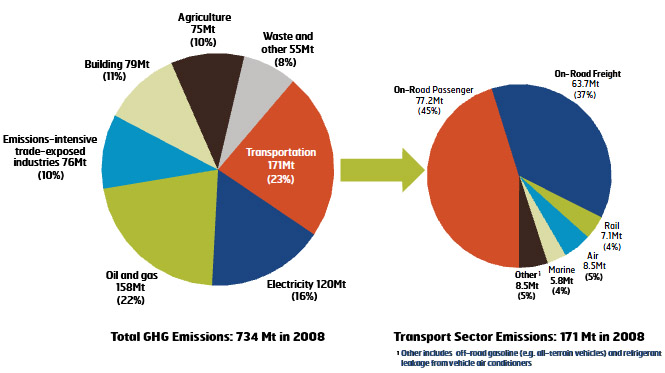
\includegraphics[height=0.28\textwidth, trim=0.2cm 0.2cm 0.2cm .2cm,clip=true]{figures/reduce_gas_emissions2.jpg}}
	\:
	\subfigure[Historical and projected reductions in $CO_2$ Emissions as provided by Transport Canada]
   {\label{fig:CO2}	   
   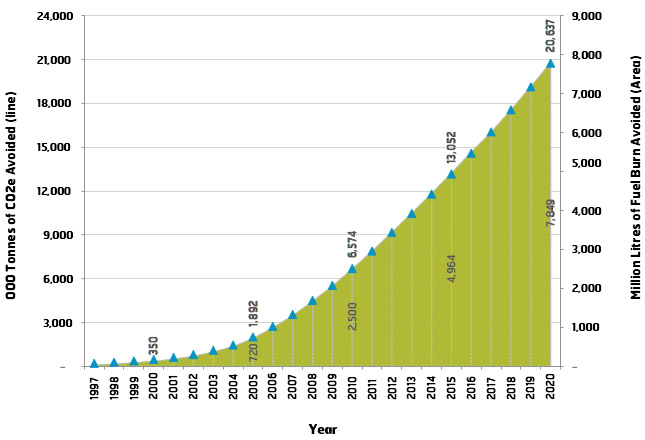
\includegraphics[width=0.45\textwidth, trim=0.2cm 0.2cm 0.2cm .2cm,clip=true]{figures/reduce_gas_emissions.jpg}}%
    \caption {\href{https://www.tc.gc.ca/media/documents/policy/AviationGHGActionPan_Eng.pdf}{Aviation and Emission}}  
\end{figure}

Presently, there is heavy emphasis on the control of pollution from the aviation sector, since it is a fast growing industry, projected to grow at an annual rate of 3-4\%. 

Engine manufacturers are continuously improving and refining engine design. An interesting observation is that there is current emphasis on reduction of $NO_x$ emissions. Within the engine, $NO_x$ formation ocues via the Zeldovich mechanism primarily in diffusion (non-premixed) type combustors. Diffusion type flames have a high primary zone temperature, which increases the production of thermal $NO_x$. The trend now is to implement partial-premixing, (i.e. mixing of air with fuel prior to entry into the combustion chamber, reducing the primary zone temperature, and consequently $NO_x$. However, the adverse effect is an increase $CO_2$ and Unburned HydroCarbons (UHCs) emission. It is difficult to pit a pollutant against another, but based on time effects, $NO_x$ has a projected lifespan of approximately 2 weeks, while $CO_2$ nearly 200 years. $CO_2$ is a greenhouse gas that effectively raises the Earth's average temperature, and rather unfortunately, takes a very long time before it is re-absorbed.\par

Other pollutants such as $NO_x$, Aircraft Induced Cirrus are also harmful, however, $CO_2$ will be considered a principal target for emission reductions, in this day and age when global forest cover is reducing. The focus thus shifts to what can be currently done to reduce emissions from Aviation. \par\par

Many governments have undertaken efforts to actively reduce aviation emission in a bid to control the surge in air travel movements, by modifying some of the standard practices. These could include allowing encouraging shorter taxi times at busy airports, charging airlines on Carbon Taxes, as well as regulatory bodies such as the Federal Aviation Administration regulating noise pollution.\par 

%%=====================================================================================================================
\section{Motivations for Continuous Descent Approach (CDA)}
\label{sec:CDA}
Continuous Descent Approach, applicable to the descent and approach phase of a flight, has been proposed as a technique for fuel reduction and noise abatement ( especially in the vicinity of the airports). This is achieved by modification of the Standard Arrival Route (STAR). The STAR is defined by ICAO as a standard Air Traffic Services (ATS) route identified in an approach procedure by which aircraft should proceed from the en-route phase to an initial approach fix. When close to this approach fix, the pilot typically receives vectoring from Air Traffic Control (ATC) to guide the aircraft to the initial waypoint of the ILS prior to landing.\par

Cao, Rathinam and Sun \cite{Cao:2011} describe the CDA as keeping the aircraft cruising at a relatively high altitude as long as possible. When arriving at the top of descent (TOD), the aircraft descends along a smooth slope with engines running at idle or near-idle settings which require significantly less engine thrust. Compared to the conventional step-down descent, the CDA reduces fuel consumption, emission, and noise impact by avoiding low altitude
(between 3,000 ft and 10,000 ft) level flight before intercepting the final 3 degree glidepath (normally 8 to 25 nautical miles away from the touchdown depending on local circumstances). It also saves flight time due to the longer high altitude cruise with high speed. However, regardless of the environmental benefits,
to date the CDA has yet been a nationwide practice due to airport safety and efficiency concerns. The near idle throttle settings makes the descent trajectories less predictable. As a result, air traffic controllers (ATCs) have to block large chunk of airspace to separate the landing aircraft. This leads to a reduction in
the throughput of an airport. So far, the CDA has been practiced only in low-density conditions or applied to a selected portion of inbound traffic in the nighttime hours rather than on a standard terminal airspace operation basis.

The STAR has a typical staircase/cascade profile as the aircraft would descend in stages along assigned waypoints, maintaining the regulated speed and altitude restrictions. This translates to flying at lower altitudes at lower speeds requiring early deployment of high-lift devices. This typically results in increased extra fuel-burn due to more power demand on the engines, as well as engine and airframe noise that would affect the surroundings near the airports.\par
\vspace{-0.8mm}
\begin{figure}[!h]
\centering
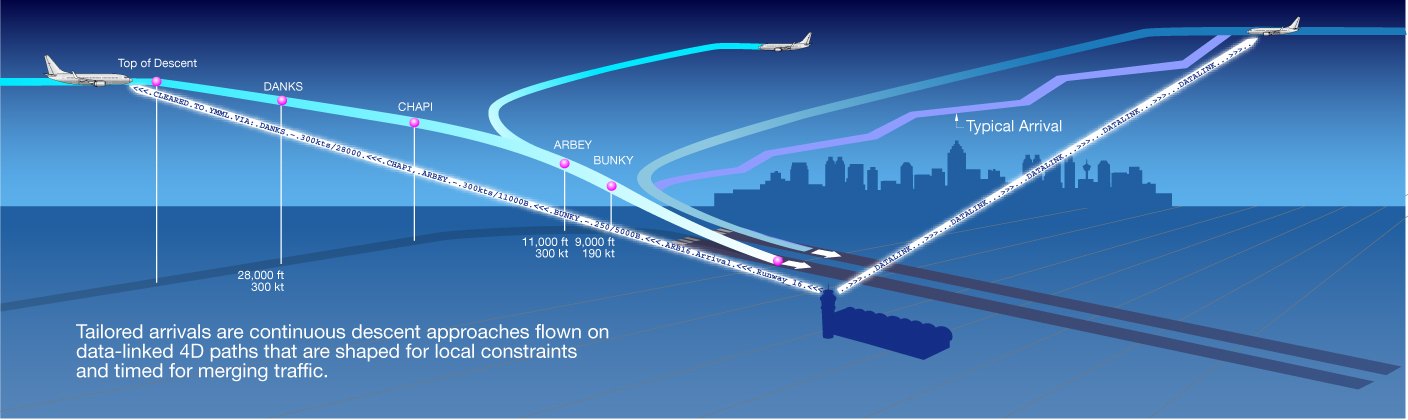
\includegraphics[width=1\textwidth]{figures/Tailored_Arrivals_YMML.jpg}
	\caption{Comparison of a STAR and TA profile at Melbourne International (YMML)}	
	\label{fig:Compare}
\end{figure}
\vspace{-0.8mm}
In the mid-1970s, British Airways began constant angle descents into Heathrow Airport, from an initial height of 7000 ft above ground level, mainly aimed towards noise reduction. CDA has been developed to begin from the cruise altitude, enabling a smooth profiled descent into the airport. CDAs are part of the larger Tailored Approaches (TA), the term more commonly used in the USA.\par
\begin{figure}
\centering
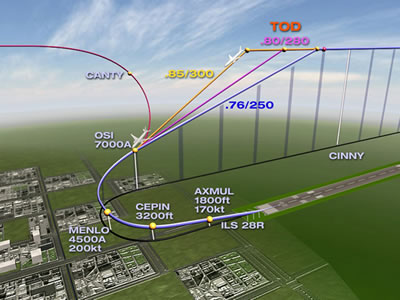
\includegraphics[width=0.45\textwidth]{figures/ils28R_tailored.jpg}
	\caption{A tailored approach into San Francisco International Airport (KSFO) Runway 28R}	
	\label{fig:KSFO ILS 28R}
\end{figure}
Major Airports that have implemented the CDA/TA include:
\vspace{-2.4mm}
\begin{enumerate}
\itemsep-0.5em
\item Los Angeles International (KLAX)
\item Heathrow International (EGLL)
\item Hartsfield-Jackson International (KATL)
\item San Francisco International (KSFO)
\item Louisville International (KSDF)
\end{enumerate}
\vspace{-2.4mm}
Some of the benefits as reported by Airlines that participated in the KATL study reported fuel savings of approximately \href{http://www.gtresearchnews.gatech.edu/continuous-descent/}{300-1000 pounds of fuel}. Since the CDA has a smooth glide profile, aircraft engines do not throttle up and down reducing the noise and emissions. Keeping engines at idle power can cut emissions of nitrogen oxides by nearly a third, and reduce noise along certain portions of the flight path prior to the Initial Fix point. CDA also has the benefit of being faster, saving a few minutes during the descent and landing phase of the flight.\par

Air New Zealand (ANZ) and QANTAS \cite{Copp:2007} participated in the \href{http://www.airways.co.nz/documents/Aspire-Annual-Report.pdf} {ASPIRE} program, which aimed at having actual commercial flights that served as demonstrations  to set an "Ideal Flight" benchmark metric. On 12 September 2008 the inaugural test flight, an ANZ-operated Boeing 777 demonstrated the capabilities of the most advanced Air Navigation Services and airline fuel optimisation initiatives in current operation. This flight had all practical operational restraints removed: including air traffic congestion control vectoring, air traffic fixed route structure, procedures, flow restrictions and airline restraints. This flight had 3.5 tonnes fuel savings (11.2 tonnes $CO_2$ reduction). One month later Qantas flew a new A380 from KLAX -YMML saving 8.9 tonnes fuel (28 tonnes $CO_2$). Although idyllic, these flights served as a benchmark for achievable savings, to which CDA contributed. \par

%%===================================================================================================================
\section{Case Studies Summary}  \label{sec:case studies}

This report analyses the works of several researchers as listed out in the bibliography. In specifics:
\begin{itemize}
\item Park and Clarke \cite{Park:2015} look at the performance bounds of CDA procedure via optimal vertical trajectory generation problems with respect to flight time and fuel consumption. Using two different types of aircraft (Boeing 737 and Boeing 767) in a numerical study, they compare the optimal CDA trajectories with a typical vertical navigation (VNAV) CDA trajectory used in CDA applications at several airports. They divide the optimal CDA vertical profile into two segments: the cruise segment before the top of descent (TOD) and the descent segment from the TOD. The descent section is further subdivided based on flap setting and speed constraints. 

\item Cao et al \cite{Cao:2013} Approach this topic from the perspective that studies which examine fuel savings from CDA
fail to consider the increased separation uncertainties that it often necessitates. They mention that this may cause extra
fuel consumption for safe spacing. Their study evaluates the fuel benefits of CDA at Atlanta Hartsfield-Jackson Airport taking into account the delays resulting from conflict resolutions. They estimate fuel burn using a corrected Thrust Specific Fuel Consumption model that is designed specially for descent. Conflict-free CDAs are determined in such a way that the total arrival
delays are minimized in each look-ahead time window. Resultant delays are converted to speed advisory or air holding commands executed in cruise phase to account for the impact of increased separations in CDAs. The fuel consumption of CDA is compared with that of real step-down trajectories extracted from radar track data. 


\item Jin and co-authors \cite{Jin:2013} also focus on the evaluation of the continuous-descent approach as a fuel-reduction procedure. Their research gives insights into the reasons why the continuous-descent approach saves fuel, and they derive design guidelines for the CDA procedures based on fuel burn dependency on speed and altitude. Their basis is the theoretical analysis that speed profile has a substantial impact just as important as vertical profile on the fuel consumption within the terminal area. In addition, the CDA is not intrinsically a fuel-saving procedure: it is contingent on conformity to the speed schedule. Based on this model, the potential fuel savings due to the CDA at the San Francisco International Airport (KSFO) are estimated, and the accuracy of this estimation analysed.

\item Mur\c{c}a and M{\"u}ller \cite{Murca:2015} present an optimization approach for dynamically scheduling aircraft operations and supporting air traffic controllers in both determining and implementing operationally feasible landing and departure times at an airport. They use a programming model to incorporate air traffic control infrastructure in terms of route network. Their model also introduces the concept of alternative approach routes and is designed to generate an output that can be converted into effective advisories for executable flight commands. It shows reasonable computational times for obtaining the optimal solution and delay reductions of up to $35 \%$ with practical size instances from Sao Paulo/Guarulhos International Airport (SBGR).

\item Takeichi and Inami \cite{Takeichi:2010} discuss the arrival-time controllability of the tailored arrival paths determined by the top-of-descent and waypoint positions. They consider a tailored arrival path which is designed using the least number of track-to-fix and radius-to-fix legs neglecting the engine thrust. They investigate two types of tailored arrival paths; one determined by adjusting the waypoint positions with the fixed top of descent, and the other determined by top-of-descent position with the fixed waypoints. These are numerically analyzed so as to satisfy a set of appropriate boundary conditions both at the top of descent and landing, and the behavior of the arrival-time difference from the standard continuous descent approach path is explored using a representative set of inputs. The arrival-time controllability is defined as the differences between the fastest and the slowest arrival time. Through several series of arrival-time analyses, it is found that the tailored arrival paths determined by changing the waypoint positions can achieve the larger arrival-time controllability compared with those determined by changing the top-of-descent position. It is also suggested that it is possible to compose an arrival path with the maximum arrival-time controllability without any additional fuel consumption.


\item Turgut et al \cite{Enis:2010} analyze the impact of CDA on fuel consumption, noise and emission.


\item Cao, Rathinam and Sun \cite{Cao:2011} present a rescheduling method for solving the conflicts between arriving aircraft which fly their preferred descent paths using the continuous descent approach. Their work is based on the 4-D trajectory concept: each aircraft calculates its 4-D trajectory and the Estimated Time of Arrival before initiating descent procedure, and reports the 4-D trajectory to the terminal area controllers at the destination airport. The reported 4-D trajectories are used for arrival sequencing. The objective is to minimize the total delay while keeping the inbound traffic conflict-free. The rescheduling problem is formulated as a Linear Program and solved with a solver, which provides as a solution the delay assignments which aircraft use to adjust the arrival time for conflict avoidance. A minimum in-trail separation is imposed between successive arrivals to meet the arrival rate of the airport. Their proposed approach leads to a conflict-free inbound traffic. Most importantly, it benefits the continuous descent approach in a sense that the conflicts are solved without changing the user-preferred trajectories, and the CDA trajectories are keep intact. 


\item Coppenbarger et al \cite{Copp:2007} discuss operational trials that were completed in January 2007 involving trans-pacific flights into San Francisco during early morning hours. Trajectory-based clearances were transmitted by datalink to Boeing 777 aircraft equipped with Future Air Navigation System avionics. NASA’s prototype, ground-based automation for high-density arrival management tailored trajectory clearances to accommodate artificially imposed metering constraints. 

\item Robinson and Kamgarpur \cite{Rob:2010} estimate the potential benefits of continuous descents for more than 480,000 flights to 25 major airports in the U.S. National Airspace System. While reduced fuel consumption and greenhouse gas emissions are expected for these procedures, the benefits during periods of congestion are not well understood. To address this gap, they constructed baseline trajectories  from flight plan and track data for flights arriving at 8 busy terminal areas. They modelled two types of continuous descent trajectories: One enforcing a constant distance-to-fly constraint to simulate uncongested operations, while the other enforcing a constant time-to-fly constraint to simulate congested operations. They calculated potential fuel savings for different continuous descent scenarios. 

\item Nikoleris and co-authors \cite{Niko:2012} compare fuel consumption of alternative descent trajectories (from cruise altitude to meter fix) when the required time of arrival is later than the nominal time of arrival at the meter fix. The required delay, i.e. the difference between the nominal and the required times of arrival, can be achieved by either slowing down the aircraft in the cruise and descent phases or flying a longer route at a constant altitude. Performance models for ten different Boeing and Airbus aircraft, were obtained from Base of Aircraft Data, and used to generate results. 

\item Hayashi et al \cite{Hayashi:2011} propose an Efficient Descent Advisor (EDA) as a ground-based decision-support tool for Air Route Traffic Control Center (ARTCC) sector controllers for managing arrival flows. This work is based on Coppenbarger et al \cite{Copp:2010b} Their tool calculates the maneuver instructions for an arrival flight to fly a conflict-free (when able), fuel-efficient, continuous-descent trajectory and also meet a time-based metering requirement at the Terminal Radar Approach Control (TRACON) boundary. As of the time of writing of their paper, speed variations and path-stretch maneuvers were the only degrees of freedom used by EDA to find a solution. Their study examined the feasibility of altitude change as an additional degree of freedom. 

\item Alam and co-authors \cite{Alam:2010} investigate the benefits of CDA with change in traffic conditions and variable noise abatement rules and consider throughput capacity of transition airspace for multiple flights performing CDA operations.


\item Coppenbarger et al \cite{Copp:2010b} present an overview of development and testing of ground-based automation for accommodating fuel-efficient arrivals in heavy traffic, this work serves as a foundation for Hayashi and co-workers\cite{Hayashi:2011}. They define the Efficient Descent Advisor (EDA), an emerging decision-support tool for air-traffic controllers managing arrival airspace in enroute facilities. It generates trajectory-based clearance advisories that allow a continuous descent at low engine power while avoiding conflicts and maximizing arrival throughput. Findings from several human-in-the-loop simulations and a field test are presented and discussed, which pertain to controller use and acceptance of EDA as a near-term capability for the Next-Generation Air Transportation System (NextGen).

\end{itemize}


%%%===================================================================================================================
%\section{Methodology} \label{sec:methodology}
%
%This section contains a summary of the case studies referered to in \ref{sec:case studies}:
%
%\begin{itemize}
%
%\item Park and Clarke \cite{Park:2015} consider the most efficient way to control high-traffic CDA minimum separations: one, using a previously developed tool for analysis of separation and throughput; and, second, to assign a required time of arrival (RTA) at a meter fix for each aircraft in the Terminal Radar Approach Control (TRACON). The RTA assignment at a meter fix requires a CDA performance-bound analysis of individual aircraft for the feasible operation. For this reason, ATCs need a methodology to analyze the performance bound of the CDA trajectory depending on the aircraft types and wind conditions. An optimal control framework is useful to analyze the performance bound of the trajectory. Their method for trajectory optimization implements optimal CDA trajectories that maximize the benefits in terms of operating costs, such as fuel consumption or flight time. To obtain these optimal trajectories, they formulate problems as multiphase optimal control problems with fixed range, and consider both operating conditions and speed constraints. The altitude range considered is from the cruise altitude to intercept of Instrument Landing System (ILS) glide slope. By dividing the optimal trajectory into two flight segments, cruise and descent, they simultaneously obtain both TOD position and optimal descent path. Furthermore, they also compare the optimal trajectories to a reference CDA trajectory generated by the FMS VNAV function and propose suboptimal trajectories for a VNAV CDA based on optimal-trajectory results. The proposed VNAV CDA vertical profiles can be calculated by an onboard flight management system (FMS) computer without additional equipment.
%
%\item Cao et al \cite{Cao:2013} use as baseline the radar track trajectories, which comes from FAA Performance Data Analysis and Reporting System (PDARS). The data contains flight information, such as 4-D trajectories, flight plans, arrival fix and ground speed. They choose for study arrival patterns into Atlanta's Hartsfield-Jackson (KATL) which has two main benefits for their analysis: firstly, arrival routes have a radial treelike structure. As a result, interactions between arrival flows are minimized, which make it easier for deconfliction modeling. Second, ATL is a hub airport that accommodates a large volume of traffic each day (a large sample size improves statistical significance of data analysis). Trajectories observed from the PDARS data mostly use conventional step-down descent. To create CDA traffic, aircraft type specific information as well as ground tracks are fed into the NASA Future ATM Concepts Evaluation Tool (FACET) to synthesize CDA trajectories. FACET uses built-in aircraft performance data to propagate the vertical profile of a given aircraft type, which is typically a 3 degree glide path. The lateral path is determined by waypoints derived from either flight plans or a given geographic coordinates array. Their ground tracks are exactly the same, with only different vertical profiles. This is to ensure that the fuel consumption difference between CDA and the baseline is only a consequence of optimized vertical profiles and speed profile. The radar updates the aircraft position with an interval of around 1 minute. To obtain a finer resolution, the update interval is turned to 5 seconds in FACET simulation mode. The simulated trajectory is a smooth glide path with delayed Time Of Descent (TOD) point.
%
%
%
%\item Jin and co-authors \cite{Jin:2013} derive an analytical link between flight
%operation parameters and fuel consumption based on the base of aircraft database (BADA) total-energy model (TEM), resulting in some guidelines for the CDA design.   This link involves the relationship between procedure variables (vertical profile and speed profile) and fuel consumption. They express fuel consumption as a function of the vertical profile and the speed profile, which is fundamentally
%nonlinear. Such nonlinearity produces some nonintuitive effects,
%for instance, elevation of flight level, increasing fuel consumption.
%They use the results from this derivation will be applied to two special cases to
%provide insights into fuel consumption in the terminal area, and to
%explain the reason why the CDA typically reduces fuel consumption; as well as a case study at the San Francisco International Airport (SFO), in which the macroscopic fuel savings are estimated.
%
%
%
%\item Mur\c{c}a and M{\"u}ller \cite{Murca:2015} analyze the optimization of aircraft sequencing and scheduling for landing. Since each aircraft has to perform a specific approach route to arrive at the destination airport (STAR), their model proposed attempts to encompass part of the associated control problem taking into account these arrival routes. More specifically, a mixed integer linear programming model was developed, which seeks to minimize the cost of the deviation of the actual landing time from the target landing time in determining how each aircraft will perform the arrival route to the airport so that the separation between aircraft on final approach is guaranteed. A STAR usually consists of a fixed number of waypoints and routes linking these waypoints. They consider the landing time of an aircraft as the time it passes over the first waypoint of the STAR plus the time spent to traverse the whole arrival route, and time spent to traverse the STAR is the sum of the standard time spent if a continuous descent approach is performed with discrete delays or discrete time advances resulting from controllers’ actions to guarantee the regulated separation between aircraft. Discrete delays or discrete time advances are associated with either alternative arrival routes or holding procedures that can be performed by an aircraft. The type of the arrival route and the number of holding procedures are a controller’s decision that impacts the landing time and that is what they aim to optimize.
%
%The sequencing and scheduling decisions are made in a dynamic environment where the set of aircraft that are going to land or takeoff and the set of aircraft that has already landed or taken off are constantly changing during the time. This online process has two aspects of dynamics. First, the set of aircraft that the controllers have to schedule changes as time passes, in other words, all the flights to be scheduled are not previously known as they would be in the static case. Second, a previous scheduling decision can be updated as time passes and new aircraft enter the scheduling window such that the rescheduling potential is higher for those aircraft that are farthest from the runway. Therefore, it is necessary to link the analytical model with a dynamic approach so that it can be better evaluated and become useful in a real time situation. 
%
%They base the scheduling window and freeze horizon on time. We considered a scheduling window that is constantly updated . The freeze horizon is a multiple of the schedule window. The process is characterized as follows: the scheduled time of arrival at the airport for the flights that have estimated time of arrival within the first x minutes of the scheduling window is frozen and the arrival time at the airport for the flights that have estimated time of arrival within the last 2x minutes of the scheduling window can still be scheduled (optimized). For every x minutes, the scheduling window is then updated, encompassing a new set of aircraft with frozen scheduled time of arrival and a new set of aircraft with arrival times to be scheduled. Therefore ensuring that if a plane begins the arrival route within a time window and lands within the next time window, it will be considered in the scheduling of the next sequence of aircraft. Hence upstream and downstream flow will always be considered for scheduling and that separations will be ensured for all pairs of aircraft.
%
%
%An example of how their dynamic approach (and optimization calculations) could be used in practice as part of a decision support tool for air traffic controllers is as follows:
%\begin{itemize}
%\item First, for all the flights within range of the reference waypoint estimated time of arrival (at the final waypoint of the STAR) would be generated from a set of input parameters such as wind and speed profiles. This prediction could be made either with the information of the radar console at the air traffic control body or with the flight management system of the aircraft (in this case, the predictions could be transmitted to the air traffic control body via data link).
%
%\item Second, the model input parameter represented by the target time of arrival at the final waypoint of the STAR would be
%updated by the values determined in the first stage. The scheduled time of arrival of the flights within the first few minutes
%of the scheduling window would also be updated with the results of the previous optimization run.
%
%\item Third, the optimization procedure would be initiated. Once model gives the configuration of the STAR to be traversed and the number of holding procedures to be performed, they would be displayed to the air traffic controllers. Finally, with this information, the air traffic controllers would be able to transmit the appropriate con-
%trol instructions to the next set of aircraft which becomes the frozen fraction of the next scheduling window (their scheduled time of arrival are frozen in the next optimization run). Here it is noticeable the benefit of the output type of the proposed model in terms of decision support. Since the scheduled time of arrival is displayed in terms of control actions, air traffic controllers are supported not only in the establishment of an arrival sequencing and scheduling solution but also in the implementation of this solution.
%\end{itemize}
%
%
%Finally, they perform a Case study with real radar data from Sao Paulo/Guarulhos International Airport (SBGR) where the operations of arrivals and departures are dependent, meaning that departure flights need to be taken into account in the arrival sequencing and scheduling process.
%
%\item Takeichi and Inami \cite{Takeichi:2010} use the equations of motion to analyse the aircraft profile in the descent trajectory by performing a flight path composition comparison for standard descent as well as CDA. They then use these equations to evaluate the arrival time for various flight angles which incorporate a given approach of a certain angle towards the base leg of the flight approaching the runway. They then calculate fastest arrival times and paths that will enable this.
%
%
%
%\item Turgut et al \cite{Enis:2010} model conventional and CDA procedures in the Istanbul terminal area (TMA), which has five entry points. The real speed and the real altitude limitations were maintained on these entry points. System for Assessing Aviation’s Global Emissions research results were also used to determine the emission savings. This study was implemented for different approach routes to the Istanbul TMA. Istanbul Ataturk Airport (LTBA) has (arrivals on RWY 06 and departures on RWY 36) was used 60 percent of time, while the remaining 40 percent being on configuration arivals 24 / departures 18. For this reason, the runway 06 was chosen for arrival airliners.
%
%For numerous approach cases, after the entry points the pilots descended until the minimum altitude limits and proceeded to low-level altitudes until the Final Approach Point (FAP). However, this approach leads to more fuel consumption and takes more time according to the CDA. Furthermore, some entry points would facilitate this kind of approach with two steps  while for others four steps stair approach is required as two descents and two low-level flights. Their study modelled one single flight per entry point. For this context, B757 was selected in order to demonstrate the results of CDA procedures in terms of fuel consumption, time and emission. 
%
%With regard to fuel consumption, the descent phase has significant fuel saving potential in terms ofoperation and traffic procedure, and their model uses the engine pressure ratio (EPR) indicator to determine the thrust generated by the engines. Since the fuel consumption depends upon numerous operational parameters including weight, weather, operation, traffic conditions, etc. they set up the model in such a way that could be able to cover wide range of engine and airliner types.
% 
%\item Cao, Rathinam and Sun \cite{Cao:2011} based their work on the 4-D trajectory concept: each aircraft calculates its 4-D trajectory and the Estimated Time of Arrival before initiating descent procedure, and reports the 4-D trajectory to the terminal area controllers at the destination airport. The 4-D Trajectory Based Operations is a concept that can enhance the predictability of the CDA The reported 4-D trajectories are used for arrival sequencing. The objective is to minimize the total delay while keeping the inbound traffic conflict-free. The rescheduling problem is formulated as a Linear Program and solved with a solver, which provides as a solution the delay assignments which aircraft use to adjust the arrival time for conflict avoidance.
%
%An ideal vertical profile of CDA is simulated using the Future ATM Concept Evaluation Tool (FACET). In this concept, each aircraft has a capability to accurately follow a planned, feasible trajectory that has been agreed upon with the controllers. The operations are then based on these trajectories that specify the complete set of positions of each aircraft along with its time of arrival at each position. The realization of this concept strongly depends on the on-board FMS and a reliable datalink between the aircraftand ATCs. En route flights calculate their estimated time of arrival (ETA) and planned standard terminal arrival routes (STARs), then report to the ATCs for approval via dedicated datalink. ATCs send back the RTAs and STARs which help the FMS to fine tune the accurate ETAs. Such negotiations are initiated at least one hour before reaching the TOD, allowing sufficient time for the ATCs to sequence and merge the arriving flows. Their model has a conflict resolution model that is enabled.
%The validation consists of two simulations. In the first simulation, aircraft perform unconstrained CDAs without rescheduling. Each aircraft is navigated by the filed flight plans, and descends along the course of CDA adhering to the built-in performance database. The first simulation generates the 4-D trajectories of all flights. The conflict count obtained from this case serves as a baseline. In the second simulation, aircraft perform constrained CDAs under separation constraints and airport arrival rate constraint. As a result, majority of the CDAs are not interrupted as delay controls are finished outside the terminal area. The 4-D trajectories exported from the first simulation are fed into the re-scheduling algorithm. Once the optimization is done, the optimal delay solutions are used to run the second simulation. In both
%simulations, statistics of fuel consumption and flight time are recorded, as well as the conflict information.
%
%
%\item Coppenbarger et al \cite{Copp:2007} investigates the the Oceanic Tailored Arrivals (OTA) trials conducted over 40 days with a single United Airlines Boeing 777 flight (UAL76) in commercial service between Honolulu and San Francisco (SFO),  chosen largely because of its early morning arrival time at SFO, which avoided congested airspace conditions, thereby minimizing the likelihood of interference with other traffic. Clearance delivery was initiated approximately 700 nmi from landing in oceanic airspace controlled by the Oakland Air-Route Traffic Control Center (ARTCC), referred to as ZOA. Once loaded, the route clearance provided sufficient information for the Flight Management System (FMS) to compute a 4-D reference trajectory from the aircraft’s current position to the runway. This trajectory was then used by the FMS as the basis for its Lateral Navigation (LNAV) and Vertical Navigation (VNAV) guidance functions, which provided inputs to the autopilot. Once activated, the route clearance allowed the flight to progress with no additional pilot inputs prior to configuring the airplane for landing.  To provide a dynamic element to the OTA trajectory-based clearance, a prototype version of NASA’s EDA decision-support tool was incorporated. EDA was used to compute the maneuver solution needed to target a meter-fix crossing time constraint imposed at the Terminal Radar Approach Control (TRACON) boundary. The Efficient Descent Advisor (EDA) tool was originally designed to assist ATC in developing conflict-free arrival metering solutions under capacity constrained conditions, and for these trials was adapted to receive oceanic surveillance and flight-plan data. 
%
%
%\item Robinson and Kamgarpour \cite{Rob:2010} estimate the potential fuel savings of continuous descents for more than 480,000 flights. Arrival flights to multiple airports in multiple TRACONs were analyzed in order to encompass congested environments like New York and Atlanta. The traffic analysis was performed using NASA’s Center/TRACON Automation System infrastructure in conjunction with ARTCC and TRACON flight plan and track data. The Aviation Systems Division at NASA Ames Research Center has continuous access flight plan, track data, and weather forecasting. They analysed fuel flow and aggregated potential fuel savings by airport, arrival procedure, landing runway,
%aircraft weight-class, and traffic demand level. 
%
%
%\item Nikoleris and co-authors \cite{Niko:2012} compare of fuel efficiency for several standard descent procedures with an RTA constraint at the meter fix and consider descent procedures as typically executed in actual operations, which are not necessarily optimal from a strict fuel cosumption perspective. Thus, fuel burn results are
%generated by simulating descent trajectories using Base of Aircraft Data (BADA) performance models of popular Boeing and Airbus aircraft with specified descent procedures such as speed reduction, intermediate altitude, path stretch and fixed flight path angle. Delays ranging from 10 seconds to seven minutes are examined. In all scenarios, the aircraft is initially at an altitude of 35,000 feet and at a distance of 150 nautical miles from the meter fix. Each scenario is characterized by the amount of delay that needs be absorbed and the descent procedure used for absorbing that delay. 
%    
%\item Hayashi et al \cite{Hayashi:2011} consider the human-in-the-loop simulation experiment simulating the north-east arrival traffic flows into the Denver
%International Airport. The flights went through sectors of the Denver ARTCC (ZDV) and were eventually handed off to the Denver TRACON. Two traffic flows, merged at a meter fix. The freeze horizon was located approximately 190 nautical miles from the meter fix. A set of hypothetical published EDA profile-descent restrictions was used in the simulation. A number of computers were used to run the entire simulation.
%
%Two traffic scenarios were created by recording the live traffic data and modifying them, such as adding some over flights to increase conflicts. Scenario 1 included 36 arrivals and 31 over flights, whereas Scenario 2 consisted of 38 arrivals and 31 over flights. The arrival rate at the meter fix was 42 per hour in both scenarios to mimic a peak-time traffic load. The peak instantaneous aircraft counts during a run were in the range of 9~22  depending on how the controller handled and handed off the traffic. The minimum horizontal separation threshold parameters set in the conflict identification computation were 6 nautical miles for conflict detection and 7 nautical miles for conflict resolution. The minimum vertical separation threshold parameters were 900 feet if both aircraft were in cruise or 2000 feet otherwise. The aircraft call signs were changed each time the scenario was reused in order to reduce learning effects.
%
%Three ZDV controllers participated in the study and switched sectors after each run, while, on the flight-deck side, three instrument-rated pilots were assigned to a pseudo-pilot station for each of the three sectors, through which the pilot handled all the aircraft in the sector and any handoffs from/to a neighboring sector. The pilot participants’ main tasks were to conduct radio communications with the controllers and perform handoffs via the pseudo-pilot station.
%
%
%\item Alam and co-authors \cite{Alam:2010} develop a methodology to generate aircraft-specific dynamic CDA routes that are both laterally and vertically optimized on given objectives (noise, emission and fuel) from an Initial Approach Fix (IAF) to Final Approach Fix (FAF). These CDA trajectories are generated by discretizing the terminal airspace into concentric cylinders with artificial waypoints, and uses enumeration and elimination (based on aircraft performance envelope) from one waypoint to another to identify all the possible routes. For each transition a variety of metrics including noise, emission and fuel burn are computed. From the resulting set of possible CDA routes, those routes are identified that represent the best trade-off on the given objectives. One of these routes was then used to dynamically update the flight route for executing the CDA procedure. For noise they used the Overall Sound Pressure Level (OPSL) and for emissions they used four pollutants HC , CO , $CO_2$ and $NO_x$ . The dynamic CDA algorithm is implemented in a high-fidelity simulator for Sydney Terminal Area, and the dynamic CDA routes compared on noise, emission and fuel burn with same flight conducting a typical CDA procedure at the Sydney airport (YSSY). They also incorporated a delay algorithm which used the flights' estimated time of arrival (ETA) at the IAF and then allocated them a conflict free CDA route by searching through available routes. The approach took into account the aircraft category and corresponding time occupancy at each artificial waypoint of the proposed CDA routes and propagated any delays back whenever conflict arose. The proposed methodology is then extended to multiple aircrafts scenario, by blocking the artificial waypoints generated for the first aircraft and making them inaccessible for other aircraft for a period of time based on estimated time of arrival (ETA) of the first aircraft at its respective artificial waypoints.
%
%\end{itemize}





%%====================================================================================================================
\section{Results and Findings} \label{sec:results}



\begin{itemize}

\item Park and Clarke \cite{Park:2015} 

\begin{itemize}
\item B737 Results
The results of the B735 minimum-time and minimum-fuel optimal trajectories are as follows: if the aircraft flies along the minimum-fuel trajectory, as much as 54 kg fuels can be saved, which is about $11.88\%$ of the total fuel burned in the minimum-time case. On the other hand, if the aircraft flies along the minimum-time trajectory, we can reduce flight time by 178 s, which is a $12.16\%$ reduction in the flight time compared to the flight time needed for the minimum-fuel case. The VNAV CDA case results are
very similar to the results of the minimum-time case with a difference in fuel burn of only 5 kg and a flight-time difference of only 20 s.

\item B767 Results
Compared to the B735, the B764 is quite large and heavy; hence, the performance characteristics of the aircraft are quite different from those of the B735. Despite the large differences in the parameters, the tendencies of the B764 optimal trajectories are very similar to those of the B735 when comparing the trajectories and speed profiles  Flight along the minimum-fuel profile consumes 85 kg less fuel than in the VNAV CDA case, which is an $11.7\%$ fuel savings when compared to the VNAV CDA case. A minimum-time profile can reduce flight time by as much as 23 s when compared to the VNAV CDA case, and 161.32 s when compared to the minimum-fuel case.
\end{itemize}


\item Cao et al \cite{Cao:2013} get results that show executing CDA does not guarantee fuel savings for individual arriving flights due to conflict avoidance, but the overall fuel consumption at the airport is reduced. The estimated fuel savings is less than that observed in the terminal airspace only, because deconfliction entails extra fuel consumption for delay absorption beyond the immediate terminal airspace.

The mean value of the fuel savings of CDA with delays is 147.99 kg/flight with a standard deviation of 18.41 kg/flight. The mean value of the fuel savings of CDA without delays is 160.22 kg/flight with a standard deviation of 18.27 kg/flight. Delays results in a 12.23 kg/flight reduction in the fuel savings on average, equivalent to $7.63\%$ of the savings attributed to the CDA vertical profiles. This estimation is in accordance with the observations by a field evaluation by Coppenbarger et al.
where a 13.5 kg reduction of fuel savings per flight due to traffic was found, even though the absolute saving values may vary from 180 kg/flight to 2700 kg/flight.
This is likely due to delays which may cause a decrease in the fuel savings.

First, as the CDA retains an almost constant descent gradient, the vertical profiles a CDA flight can fly is almost fixed once its speed profile (aircraft type specific)
is selected, so is the fuel burn. But the baseline trajectories have a variety of vertical profiles with varying level-flight parameters, e.g. number of level-flights, distance of each level-flight and altitude where level-flight is executed. All these parameters are contingent upon traffic conditions and descent procedures chosen, and cause the baseline fuel burn to vary. As a result, the fuel saving numbers vary accordingly. The trends of both the mean values and the median values indicate that the savings are almost linearly correlated to the number of level flight executed. Among the presented aircraft types those with a long range flight segment showed the highest potential of savings. 


\item Jin and co-authors \cite{Jin:2013} find:
\begin{itemize}
\item The CDA eliminates level segments at low altitude by elevating them to a high altitude.
\item The CDA typically increases the average speed because in most cases, a higher indicated airspeed is assigned at a higher altitude. (the fuel-optimal cruise speed is usually higher than the actual operating speed.)
\item The CDA moves the speed profile closer to the fuel-optimal speed profile.
\item Case Study Results: Potential Fuel Savings at the San Francisco International Airport (SFO)
As expected, different speed profiles give significantly different results. The speed from radar data is usually lower than the fuel-optimal speed. As a result, a higher altitude increases fuel consumption, and thus the CDA consumes even more fuel (the radar-recorded column). The BADA-recommended speed profile yields high fuel
savings. Such difference suggests that, in the terminal area, a faster speed profile usually means less fuel consumption. A large standard deviation of fuel saved is observed, meaning that the mean values are only macroscopically valid. For a particular flight, the potential fuel savings are extremely sensitive to a number of factors, including aircraft-performance parameters, procedure parameters, and weather. The data distribution suggests that the introduction of the CDA be focused on wide-body aircraft and be avoided for those flights with negative fuel savings.
\end{itemize}

Hence, the CDA saves fuel not only by elevating level-flight altitude, but, perhaps more importantly, by increasing speed, or moreprecisely, by shifting the speed profile closer to the fuel-optimal speed. Speed influences fuel consumption as significantly as, if not more than, altitude. In other words, if a CDA procedure were designed without an appropriate speed profile, such CDA might consume even more fuel than the corresponding conventional procedure. This conclusion is further justified by the case study of a RJ-200 at the San Francisco International Airport, where the proposed CDA procedure consumes more fuel than the realistic step-down procedure.

Skillful manipulation of the speed profile could potentially be a promising strategy to fuel reduction, especially when the altitude constraint is binding. As much as 60 kg of fuel would be saved during a 10,000 m level segment at 9000 ft simply by changing the speed from 200 to 250 kt. A similar result is observed in constant-speed descent.
Although the CDA is intended to reduce fuel consumption and to abate noise simultaneously, which is the case in the high speed range (e.g., over 300 kt at 15,000 ft for the B747-400), these two objectives tend to conflict with each other in the low speed range (e.g., under 250 kt at 9000 ft).  Therefore, level flight at low speed is never recommended in terms of fuel consumption. Finally, another possible reason why the CDA saves fuel is that repeated acceleration/deceleration is largely avoided.

\item Mur\c{c}a and M{\"u}ller \cite{Murca:2015} find that the use of continuous decision variables generates a high range of different outcomes in terms of time devi-
ations to be absorbed by the aircraft, and the transmission of such information to the pilot could increase the occurrence of noise in communications as well as increase the workload of the controller, especially if a dynamic approach is used, because, at each entry of aircraft into the system, new sequences and new arrival times are determined. Therefore, in this case, the controller would still be responsible for determining the control actions (speed adjustment, altitude adjustment, holding procedure, route lengthening/shortening etc) required for each aircraft to reach the metering fix at a given time that is the closest to the optimal time resulting from the scheduling. Thus, in case of voice communications systems or in case other types of control actions are still necessary to provide the separations, especially in the terminal area, a broader underlying flow control conception (in other words, a conception that offers a range of control actions other than speed adjustment) is required. Moreover, if the air traffic controller is still responsible for implementing an arrival sequencing and scheduling solution, an optimization approach that incorporates this broader control problem becomes more appropriate. Their work has the objective to help the controller in determining the configuration of the STAR to be traversed and the number of holding procedures to be performed. The configuration of the STAR would be selected from a set of standard procedures that would have been previously tested, validated and implemented by air traffic control bodies. 


\item Takeichi and Inami \cite{Takeichi:2010}
   It is found that the arrival-time difference of the fastest fixed TOD
path becomes larger as the longer final glide path is applied. On the contrary, the arrival-time difference of the fastest fixed WP path becomes smaller. Both of the
Fixed TOD and Fixed WP fastest arrival paths are obtained when the flight-path angles coincide with the limit values. The faster arrival-time difference of the fixed WP path also decreases because the arrival-time control is made mainly by the flight-path angle of the leg. On the other hand, the faster arrival-time difference of the fixed TOD path increases because the path length difference between the standard and the fastest path length becomes larger. However the path length difference turns to decrease as the final glide-path length further increases, and the increase rate of the faster arrival-time difference becomes smaller. Both of the arrival-time difference of the slowest Fixed TOD and Fixed WP  paths are almost the same values and decrease in almost the same manner. As mentioned above, the slowest arrival path is determined so that the aircraft dissipates its mechanical energy as long as possible with satisfying the boundary conditions. Hence there are small differences between the slowest arrival times of the Fixed TOD and fixed WP paths. Because the arrival time of the standard CDA path with longer final glide path becomes larger while the slowest arrival time hardly differ, the difference between the slowest arrival time and the standard one monotonously decreases. Because the faster arrival-time difference increases with its rate decreasing, and the slower arrival-time difference monotonously decreases in the case of the fixed TOD paths, the arrival-time controllability has a maximum value. It is
possible to compose various arrival path with the same maximum controllability. Therefore, it is expected to be possible to achieve the maximum controllability and the noise abatement simultaneously by composing the arrival path avoiding residential area and achieving obstacle clearance by composing the arrival path avoiding large obstacles, such as tall buildings, mountains, etc.


\item Turgut et al \cite{Enis:2010}
With CDA procedures, more than 40 kg fuel and 2 min time savings per flight are obtained; furthermore, regarding $CO_2$ and $H_2O$, significant emission savings are also noted.  The effects can be grouped in two main titles since the main estimated benefits are fuel and emission. There is also another benefit in which revealed as time, which was attributed into the energy part.

\begin{itemize}
\item Energy management aspect

Considering the five entry points, 7-9 percent of fuel savings are obtained. The largest saving is observed at entry point BIG as 44 kg, since this entry point has the longest level flight distance as 55 nm. However, the lowest fuel saving is obtained at YAA as 27 kg for a level flight distance of 30.4 nm. Despite the fact that the level flight distance is directly proportional with the fuel burned, the other important factor is the percentage of how many miles are flown at relatively higher altitudes. For this reason, considering the EKI (35 nm) and YAA (30.4 nm), one can see that despite difference of almost 5 nm and also the level flights at the same altitudes (6,000 and 3,000 ft), the fuel savings (or fuel burned) are quite close to each other. The reason could be explained in such a way that in EKI the level flight distance at 6,000 ft is 10 nm, while in YAA it is only 5.4 nm. Therefore, in EKI, since the distance difference of 4.6 nm (35-30.4) is flown at high altitudes, the fuel burned is maintained at modest level according to the YAA.
  Effects of CDA on the flight durations reduction are in the range of 17.8 and 19.3 percent by CDA, which correspond up to 2.8 min. Considering the investigated conditions (descent from the altitude of 37,000ft requires 25.5 min for a distance of 125.8 nm), it is revealed that the amount of savings which could be around 10 percent of the total descent duration is significantly high.  Furthermore, the fuel savings are not only acquired from the reduction of the descent time, but also from the elevating the level flight altitude, which addressed the low-power usage.

\item Emission management aspect
The amount of emission is directly proportional with the fuel consumption, while the altitude that these emissions are produced has further impacts (i.e. greenhouse effects), which were kept out of the scope of their study. 

\end{itemize}

\item Cao, Rathinam and Sun \cite{Cao:2011} 
Simulation results revealed that their re-scheduling algorithm is able to de-conflict all the arriving aircraft with different prescribed horizontal separation settings in a full day terminal airspace operation at Newark Liberty International Airport. The runtime of the algorithm is within a reasonable time horizon. Benefits analysis indicates that 80 tonnes fuel and 638 minutes flight time are saved as a consequence of employing the conflict-free CDA. Compared to the conventional step-down approach, CDA reduces the flight time as well as fuel consumption. Statistical analysis reveals that total 80,027 kg fuel (110 kg/flight) and 638 minutes flight time (53 sec/flight)
are saved (with D = 5 nm) if the step-down descents are changed to CDAs in a full day operation. As a trade-off, a total delay of 431 minutes is required for CDA separation. Depending on the scenario, this delay can be absorbed by delaying the aircraft either on the ground or while it is airborne. For instance, if delaying an aircraft on the ground does not add any constraints at its departing airport, then the aircraft can be held on the ground. On the other hand, if the cost due to delaying the aircraft while it is airborne is manageable, then one should consider the latter option.


\item Coppenbarger et al \cite{Copp:2007} 
A benefits analysis suggests Boeing 777 fuel savings of between 200 and 3,000 lbs per flight – depending highly upon baseline traffic conditions – together with a corresponding reduction in CO 2 emissions of between 700 and 10,000 lbs per flight.

\begin{itemize}
\item Fuel Benefits
Particularly for morning and evening flights when traffic is heaviest, their data showed the inefficient lateral vectoring and altitude level-off maneuvers resulting from air-traffic control actions taken to manage separation and throughput constraints. Under light-congestion traffic conditions, results indicate average fuel savings of 242 lbs per flight over current-day baseline operations for B777 flights arriving SFO along CEP routes.  For medium and heavy traffic congestion scenarios, average estimated OTA fuel savings increase to 358 lbs and 3,219 lbs per flight, respectively. The dramatic increase in estimated fuel savings for the heavy traffic comparison
was due to the inefficiencies inherent in the baseline scenario for achieving flow management and separation
assurance under congested conditions. These inefficiencies included an extra 30 nmi path-stretch
segment performed in level flight at low altitude (6,000 ft). 
\item Emissions Benefits
Results suggest that an idle-thrust, descent to the runway can reduce CO2 emissions by 761 lbs per flight in comparison with B777 operations on similar routes
conducted during light traffic congestion. In comparison with medium and heavy traffic-congestion baselines, CDA has the potential to reduce $CO_2$ emissions by as much as 1,128 lbs and 10,137 lbs per flight, respectively. These large greenhouse gas reductions reflect the approximate 3:1 ratio between fuel burned and $CO_2$ emitted, resulting
from the basic combustion chemistry of jet fuel.
\end{itemize}



\item Robinson and Kamgarpur \cite{Rob:2010} 
Analysis of the distance-constrained trajectories showed that fuel savings was distributed unevenly among the flights. The estimated savings was less than 25 kg for over $45\%$ of the flights, and less than 100 kg for over $87\%$ of the flights. The time-constrained trajectories showed $70-85\%$ less potential savings than the distance-constrained trajectories. Prioritization of the improvements necessary to execute continuous descents during periods of congestion must rely upon analysis of a sufficient sample of operations, representative of many days, aircraft types, and traffic demand levels.
   
\begin{itemize}    
\item Variability of potential fuel savings between flights and between days was calculated in order to understand how the diversity of the traffic sample affected the results. Analysis of the potential fuel savings per flight, for the distance-constrained scenario, shows that its statistical distributions for each airport exhibit long tails. In general, the mean fuel savings per flight is $20-80\%$ greater than the median fuel savings for the same traffic sample. One cause of the disparity between the mean and median values is that fuel flow rates vary by aircraft type. Thus, whereas aircraft of the super-heavy and heavy weight-class represent approximately $8\%$ of all operations, they account for approximately $22\%$ of the potential fuel savings. Limited analyses suggest that a sample reduced to a single weight-class on the same arrival route to the same runway exhibits reduced disparity between the mean and median per flight values. In order to represent the benefit of a continuous descent to the typical flight, the median value, rather than its mean value, will be reported. Ultimately, the use of either statistic will depend upon whether the purpose is to achieve the greatest total fuel savings, the most equitable distribution of fuel savings across all flights, or somewhere in between.

\item Comparison of potential fuel savings for full and partial continuous descents were made for each airport. The median fuel savings per flight was calculated for the distance-constrained trajectories of all traffic samples using the adjusted fuel flow model. The terminal, transition, low en route and high en route level segments account
for 62, 20, 8 and $10\%$ of the potential fuel savings, respectively.  Much of this level distance is a result of delay absorption in the TRACON and procedural separation from aircraft to the nearby dominant airport (i.e., DFW, ORD, and SFO). Elimination of these level segments would require improved scheduling, as well as airspace redesign. Meanwhile, ATL, DFW, ORD and SFO have similar shares of potential fuel savings for level segments in both terminal and transition airspace. The results for the partial continuous descent scenarios, whose level segments were replaced with level segments at the key altitudes instead of the cruise altitude, showed approximately half of the savings as the full continuous descent scenarios. This indicates that partial continuous descent scenarios (i.e., ones that initiate the continuous descent from higher intermediate altitudes instead of from cruise altitude) should be investigated as an alternative if a costly airspace redesign or infrastructure improvements must be avoided.

\item Comparison of potential fuel savings for distance-constrained and time-constrained trajectories. Level segments after descent from cruise altitude are associated with a time penalty, as well as a fuel penalty. Elimination of the level segments at intermediate altitudes decreases the flight time from top-of-descent to landing,
because flights are able to maintain faster speeds at the higher altitudes. The median time savings per flight was calculated for the distance-constrained trajectories of all traffic samples using the adjusted fuel flow model. The result was a median flight time savings of approximately two minutes. The 25th percentile and 75th percentile values were approximately one minute and three minutes, respectively. The estimated fuel savings per flight for the time-constrained trajectories were $70-85\%$ less than the estimated fuel savings per flight for the distance-constrained trajectories.
\end{itemize}


\item Nikoleris and co-authors \cite{Niko:2012} 
They demonstrated that the most fuel-efficient speed control procedure for absorbing delay is reducing descent speed as much as possible and then reducing cruise speed (a common finding for all ten aircraft considered). They also show that when delay is entirely offset by speed control, fuel consumption of the resulting trajectory is less than that of the nominal trajectory. For some aircraft, flying at a fixed flight path angle and constant Mach/calibrated-airspeed results in lower fuel consumption compared to standard descents at idle-thrust and constant Mach/calibrated-airspeed. Finally, for the cases examined, it is shown that executing a path stretch maneuver at 35,000 feet altitude and continuing to descend at a reduced speed is more fuel efficient than inserting an intermediate-altitude cruise segment.

\begin{itemize}
\item Idle-thrust Descent at Constant Mach/CAS
Descent at idle-thrust and constant Mach/CAS is the most common descent procedure employed by pilots of large jets.  The descent portion of the trajectory in these four methods is conducted at idle-thrust. For example, the cruise-only method and the descent-only method cannot be used to absorb delays greater than 70sec and 110 sec, respectively, given a minimum Mach of 0.71 and a CAS of 250 knots. Cruise-first and descent-first methods can be used to absorb larger delays. Note that the cruise-
The descent-first method is the most fuel-efficient method for the entire range of delays. Reducing descent CAS first results in more time spent in idle-thrust condition compared to reducing cruise Mach first, which results in more time spent at higher thrust. The descent-first method was found to be the most fuel efficient. Moreover, the descent-only procedure results in trajectories with lower fuel burn than the nominal trajectory. The aircraft spends more time on idle-thrust setting and less at higher cruise thrust compared to the nominal trajectory. This results in lower fuel consumption.

\item Constant Flight Path Angle Descent at Constant Mach/CAS
These types of descents are frequently executed by regional/business jets but not by large jet transport aircraft because the vertical navigation capabilities of their FMS make it diffcult to implement this procedure. In spite of this fact, constant flight path anglefact, constant flight path angle descent at constant Mach/CAS is examined for large commercial jets. It turns out that in many instances it yields lower fuel consumption than idle-thrust descent at constant Mach/CAS.

\item Idle-thrust Descent at Constant Flight Path Angle
Although this type of descent is not commonly executed it was found to result in lower fuel consumption than idle-thrust descent at constant Mach/CAS in some instances. The procedure consists of reducing the cruise speed and flying at that speed to the ToD point. Thrust is set to idle beyond ToD and a specific flight path angle is
maintained during descent to the meter fix.  As expected, descent at the smallest slope of 800 ft every 3 nmi consumes the least amount of fuel. Longer descent segment means that the engines operate at idle for a longer duration. Comparing Fig. 14 to Fig. 10, it is seen that the shallower flight path angle descent of 800 ft every 3 nmi results in lower fuel consumption. Results for B747, B757 and B767 were found to be very similar to B737. These results suggest that idle-thrust descent at constant flight path angle has the potential of reducing fuel consumption compared to that resulting from the standard idle-thrust descent at constant Mach/CAS.
\end{itemize}

\item Hayashi et al \cite{Hayashi:2011} 
Results of the human-in-the-loop simulation experiment showed that the altitude-advisory capability reduced the number of conflicting EDA advisories. It also reduced controller workload when the traffic situation was complex. Results also suggested that changes to EDA’s user interface design and inter-sector coordination procedures are required for controllers to accept an altitude-advisory capability.
Of the flights simulated, 29 fell outside the 20-second meet-time tolerance envelope. Close investigations of these flights revealed the following five reasons for the meet-time deviations: 1) the controller manually intervened near the meter fix to adjust separation at the meter fix; 2) the pilot used the MCP instead of the FMS to comply with a cruise-speed clearance after the EDA advisory speeds were input to the FMS, which caused the FMS-programmed descent speed not to be executed; 3) the arrival flights whose |Δ| was less than the set threshold did not receive an EDA advisory, and errors built up during the descent phase, when the EDA advisory was suppressed; 4) the EDA
advisory included a sharp turnout for conflict avoidance, and errors in the turn trajectory caused a large meet-time error; and 5) occasionally, EDA was unable to come up with a corrective advisory because of trajectory-computation error, and the meet-time error was not corrected. Reasons 4) and 5) are under investigation. The remaining reasons are related to the EDA concept of operations and will be discussed in the Discussion section. When the meet-time-error data that fell outside the 20-second tolerance envelope were excluded, the average meet-time error was 3.6 seconds, and the standard deviation was reduced to 7.5 seconds.


\item Alam and co-authors \cite{Alam:2010} 
 The results shows that the methodology generates 64 possible solutions (dynamic CDA routes) from IAF to FAF in the transition airspace, of which 5 solutions were non-dominated. Dynamic CDA approach shows a reduction of $14.96\%$ in noise, $11.6\%$ reduction in NO x emission and $1.5\%$ reduction in fuel burn when compared to a standard CDA trajectory.
Throughput: Routing and interval spacing can allow the system to increase throughput when congestion occurs via certain sectors. When the inter arrival time between flights is increased througout could even be independent of the traffic distribution. 
System Delay: Increasing the inter arrival time gives the leastfor a biased traffic distribution. For an evenly distributed traffic the best performance is achieved with
an even smaller inter arrival time.
Cumulative Noise, Emission and Fuel burn: For $NO_x$ emissions, biased traffic distribution shows highest emission for inter-arrival time of 0, as it results in highest hold patterns, leading to higher fuel burn and emission. However with increased inter arrival timings of 30, 60 and 90, there is the least emission. A similar pattern is reflected in fuel burn other traffic distributions. In terms of noise, biased traffic patterns remains highest noise contributor, and can be explained by the fact that such scenarios require more spiral routing pattern in the transition airspace to accommodate for the highly concentrated traffic in one area.


\end{itemize}

%========================================================================================

\section{Conclusions}  \label{sec:conclusion}

\begin{itemize}

\item Park and Clarke \cite{Park:2015} 
\begin{itemize}
\item A CDA can reduce operating costs by reducing the flight time, fuel burn, and reducing noise and gaseous emissions. To
\item Because the proposed VNAV CDA profiles can be calculated by onboard FMS computer without additional equipment, they represent a practical implementation. 
\item The resulting performance of the VNAV CDA profile was identical to the optimal results. 
\item If the aircraft has the capability to calculate the parameter optimization, using the proposed VNAV sequence, the optimal trajectory can be calculated very quickly, and an alternative way is that a ground automation tool solves the parameter-optimization problem using the proposed VNAV sequence, and sends the optimal parameter to the
aircraft via data link. 
\item  To determine the optimal scheduling, which is the RTA, an ATC should know the performance bound of the individual aircraft, such as the feasible time range of the CDA flight. 
\end{itemize}

\item Cao et al \cite{Cao:2013}
The principal contribution of this study is that the CDAs are evaluated under increased separation constraints such that the estimation of fuel benefits takes into account ATC control.
\begin{itemize}
\item Average fuel savings for each arrival flight is 147.88kg/flight, falling within the range of the IATA reported number 50~200 kg/flight. Individual
negative fuel savings are also observed. But, airport wide, CDA is still fuel efficient. 
\item The fuel savings is less than that observed during the descent phase only. A 12.23 kg/flight reduction in the fuel savings is found due to the delays resulting from a deconfliction algorithm. 
\item It is also found that the increased separations have a significant impact on the delays calculated. Such impact potentially decreases airport throughput, thus can be deemed as a tradeoff of use of CDA as a terminal operation procedure.
\end{itemize}


\item Jin and co-authors \cite{Jin:2013} 
\begin{itemize}
\item The case study for the San Francisco International Airport (SFO) yields multiple design guidelines on the development of the CDA procedures, which involve the arrival procedure for individual flights and suggest the priority of some aircraft types over others. The estimated fuel savings are a valuable reference for policy making, and can be consulted for estimation at other airports with comparable throughput and importance.
\item Fuel consumption in the terminal area strongly depends on the approach procedure, or, specifically, the vertical profile and speed profile. The relationship among fuel consumption, altitude, and speed is neither linear nor monotonic. At low speeds, fuel consumption increases with altitude, but decreases with speed. At high speeds,
fuel consumption decreases with altitude, but increases with speed.For a given altitude, there is, in most cases, a fuel-optimal speed that minimizes fuel consumption.
\item The CDA typically reduces fuel consumption by increasing cruise (or level flight) altitude as well as by increasing speed. If an excessively low speed profile were
assigned to a CDA procedure, the CDA procedure would consume even more fuel than its conventional counterpart. To maximize the fuel savings due to the CDA, the speed profile has to be designed as appropriately as the vertical profile. As a result, the estimation of potential fuel savings due to the CDA strongly depends on the speed
profile. 
\item Wide-body aircraft should be the target group of the CDA design because their fuel consumption would be considerably reduced through well-designed CDA procedures, and because unsatisfactory CDA procedures could result in a remarkable increase of fel consumption. 
\item In terms of maximizing the CDA’s environmental benefits, it seems that the approach procedures of narrow-body aircraft can be sacrificed for optimized CDA procedures of wide-body aircraft: deconfliction of the CDA for narrow-body aircraft is no easier than that for wide-body aircraft, but it gives few environmental benefits due to the low fuel flow rate of narrow-body aircraft. 
\item As a result, the CDA should be applied to wide-body aircraft, and the CDA of narrow-body aircraft is neither favorable nor necessary. (PLEASE MAKE A NOTE TO CRITIQUE THIS VIEW!!!!!!!!!!)
\end{itemize}



\item Mur\c{c}a and M{\"u}ller \cite{Murca:2015}

\begin{itemize}
\item The model introduces the concept of alternative arrival routes, ties the arrival sequencing and scheduling to the configuration of the terminal area in terms of Standard Terminal Arrival Routes and generates an output that is directly linked to executable flight commands. 
\item    A real case study was used to analyze the performance of the model under different operating scenarios in terms of computational tractability and delay reduction potential. For this, we used a radar database of a typical day of operations from Sao Paulo/Guarulhos International Airport (SBGR). The results show reasonable computational times for obtaining the optimal solution within feasible computational times if the dynamic approach developed is implemented in a real time situation.
\item  Also, the results show delay reductions of up to $35\%$ for the scenarios that are the closest to the actual operations of SBGR. It is worth noting that the results in terms of computational time are affected by CPLEX performance and they will vary if other solvers are used. However, it is also possible to attempt to develop heuristics for obtaining good solutions, close to the optimum, with smaller computational times.
\item Air traffic controllers can be supported both in the establishment and in the implementation of an arrival sequencing and scheduling solution.
\end{itemize}


\item Takeichi and Inami \cite{Takeichi:2010}
\begin{itemize}
\item Fixed TOD paths can achieve the larger time controllability than the fixed WP paths. In addition, it is possible to control the arrival time of the fixed TOD
path without any additional fuel consumption, in contrast to the conventional fixed WP path which inevitably requires the additional fuel consumption for faster arrival-time control.
\item It is possible to maximize the arrival-time controllability of the TA operation by having aircraft arrive toward the TOD of the arrival path with the maximum controllability, and indicating a TA path to satisfy the required time of arrival: it is further possible to compose the standard arrival route considering other conditions, such as the noise abatement, the obstacle clearance, etc. 
\item Through the arrival-time analyses, it has also been shown that it is possible to compose the faster arrival path by the fixed TOD path without any additional fuel consumption, and that it is possible to compose the slower arrival path by the fixed WP path with reducing the fuel consumption. Therefore the simultaneous optimization of the arrival-time controllability and the fuel reduction is also possible by the combination of the faster fixed TOD path and the slower fixed WP path.
\end{itemize}


\item Turgut et al \cite{Enis:2010}

\begin{itemize}
\item For almost 35,000 flights, the fuel savings could be calculated as 1 M kg/year due to the minimum result of this study as 27.3 kg for the YAA case. 
\item Savings for the other emission species such as NOx, CO and HC would have significant values as 24,500 kg for NOx, 2,625 kg for CO and 280 kg for HC according to the example given above.
\item The fuel savings for a single airliner is obtained as up to 44.3 kg for switching from the conventional to CDA procedures. This saving is occurred mainly by flying higher altitude, which leads flying against to less drag force. Time savings is also seen with a maximum value of 2.8 min since the airliner would fly faster at higher altitudes. 
\item In comparing with other studies, the results of fuel savings were found seem relatively low. In conclusion, fuel consumption is a very complex function of
many factors impacted at the same time. Therefore, comparison of results tested at different conditions could not provide consistent results between each other. 
\item Traffic density is the main limitation to obtain these savings. Although, there are some ongoing researches to use CDA procedures at heavy traffic airports without any negative impact over both the controller and the pilots currently they do not seem technically viable. The main goal of these studies is to solve the problem with integrating highly computerized FMS and to use exclusive software to which intends only optimizing the traffic problems. 
\item A good CDA procedure must satisfy three groups, which are controllers, pilots and the airline itself. 
\end{itemize}


\item Cao, Rathinam and Sun \cite{Cao:2011} 
\begin{itemize}
\item  A re-scheduling algorithm is proposed to strategically solve the conflicts between the arriving flights flying the CDAs. This approach separates the aircraft by rescheduling their times of arrival at the boundary of the terminal area. A minimum in-trail separation is imposed to guarantee the capacity benchmark rate of the airport is not violated. 
\item Simulation results verify that, in a single airport scenario, all conflicts can be solved with a reasonable runtime, and the airport capacity is well respected. Compared to other conflict resolutions, this approach does not require tactical maneuvers which potentially disturb the CDA procedure. Although it results in delays, the savings of fuel and flight time at the terminal area render such delays a minor trade-off.
\end{itemize}


\item Coppenbarger et al \cite{Copp:2007} 
\begin{itemize}
\item   The San Francisco Oceanic Tailored Arrivals field trials demonstrated the ability to conduct highly efficient CDA operations under real-world conditions with commercial airplanes. By integrating advanced air and ground automation over datalink in oceanic airspace, these trials provide a step towards understanding the feasibility and benefits of conducting trajectory-based arrival operations under NextGen. To progress towards enabling Tailored Arrivals under congested traffic conditions where benefits are greatest, NASA’s ground-based EDA automation was used to tailor trajectory solutions to accommodate time-based metering constraints. Data gathered during these trials was used to perform an assessment of EDA trajectory prediction accuracy and precision in comparison with FMS predictions and surveillance truth data. 
\item Results show that trajectory prediction errors can be greatly reduced through the uplink of wind and descent-speed-intent data, and that similar arrival-time prediction performance can be achieved between air and ground automation. 
\item These results are important because accurate and compatible prediction performance between air and ground automation is fundamental to both the planning and execution of trajectory-based arrival operations. 
\item An initial benefits assessment based on the real-world data gathered during these trials shows substantial per-flight reductions in fuel burn and environmental emissions afforded by Tailored Arrivals, especially in comparison with baseline arrival operations conducted under heavy traffic conditions. 
\end{itemize}

\item Robinson and Kamgarpur \cite{Rob:2010} 
\begin{itemize}
\item First, the estimated fuel savings are found to be sensitive to the size (e.g., number of days, flights, etc.) and diversity (e.g., proportion of different weight-classes, arrival routes, etc.) of the traffic samples analyzed. The potential fuel savings of an airport’s worst day appeared twice as large as that of its best day. The variability between flights of the potential fuel savings illustrates that simple statistical measures (i.e., mean and total fuel savings) do not adequately describe the fuel savings of continuous descents for the typical flight. In particular, aircraft of the super-heavy and heavy weight-classes were approximately $8\%$ of the total operations, but they were approximately $22\%$ of the predicted fuel savings.
\item Second, the estimated fuel savings are significantly affected by the choice of fuel flow model and continuous descent scenario. Different airports exhibit
markedly different distributions. Thus, extrapolation of the estimated fuel savings of one airport to other seemingly comparable airports, on the basis of simple characteristics (e.g., number of operations, perceived complexity, etc.), will not capture the uniqueness of each airport’s operations, or hence its potential fuel savings.
\item Third, the typical flight’s estimated fuel savings associated with eliminating level segments below 17,000 feet MSL was modest. The duration of these level segments was less than 25 nmi for $52\%$ of the flights. Also, the level distance showed considerable variation between airports; only $16\%$ of SFO flights had level distances greater than 30 nmi, while $58\%$ of ORD flights did. Elimination of these level segments accounted for approximately $80\%$ of the fuel savings estimated for full continuous descents from cruise. Furthermore, the estimated fuel savings was not distributed evenly among flights. It was less than 25 kg for more than $45\%$ of flights, and less than 100 kg for more than $87\%$ of the flights. As a result, $13\%$ of the flights accounted for $37\%$ of the total fuel savings.
\item Lastly, the estimated fuel savings were not found to scale with traffic demand, and they showed diminished returns when delay needed to be absorbed in the form of level segments. The median level distance below 17,000 feet MSL increased by approximately 10 nmi between low and high traffic demand conditions. However, it did not
show a strong trend between moderate and high traffic demand conditions for some airports. Enforcement of the time constraint on the continuous descent trajectories reduced estimated fuel savings by up to $70-85\%$. The reduction of potential benefits would be most severe when the delay required to be absorbed was the greatest.
\item Finally, continuous descents have demonstrable fuel savings, especially when executed during periods of low to moderate traffic demand. Many studies have consistently indicated that the potential fuel savings per flight is between 50 and 150 kg. However, the magnitude of these benefits, and their importance, depends upon the context
in which they are described. For example, the fuel savings associated with continuous descents, as a fraction of total fuel consumption, was estimated to be approximately $3\%$. This fuel savings equates to less than $1$ USD per passenger for a typical single-aisle, narrow-body jet aircraft. Ultimately, the NAS improvements needed to conduct
continuous descents during periods of high traffic demand will incur substantial costs to develop advanced ground automation, create new arrival procedures, and redesign existing airspace structures. Therefore, the prioritization of these improvements must rely upon an analysis of a sufficient sample of operations that is representative of many days, aircraft types, and traffic demand levels. 
\end{itemize}


\item Nikoleris and co-authors \cite{Niko:2012} 
\begin{itemize}
\item Four speed control techniques were considered for absorbing the delays needed for meeting the required time of arrival constraint at the meter fix with idle-thrust descent at constant Mach/calibrated-airspeed, namely cruise-only, descent-only, cruise-first and descent-first. Of these four techniques, the descent-first method, in which
the descent calibrated-airspeed is reduced first to absorb as much delay as possible and then cruise Mach is reduced to absorb the remaining delay, turned out to be the most fuel efficient procedure for a wide range of delays.
\item  The constant flight path angle descent at constant Mach/calibrated-airspeed, a procedure used by regional and business jets but not by large jets, was found to be more fuel efficient compared to the standard descent procedure at idle-thrust and at constant Mach/calibrated-airspeed. The difference in fuel consumption with these two procedures ranged between $-8\%$ and $+10\%$.
\item  Furthermore, comparison of 1) path stretch at high altitude and 2) descent without path stretch that includes cruise at an intermediate altitude led to the conclusion that the best approach from fuel consumption perspective is to cruise at minimum speed, complete a path stretch at high altitude at that minimum speed, and then descend at minimum speed. This method is also used in the Efficient Descent Advisor to generate advisories for meeting the required time of arrival at the meter fix.
\end{itemize}



\item Alam and co-authors \cite{Alam:2010} 
\begin{itemize}
\item  All the routes in this set show the trade-off between the competing objectives of noise, emission and fuel burn. By assigning desired weights based on operational
priority of each objective and using a simple search algorithm, the desired route can be selected for uplink to the aircraft's FMS. These waypoints can then be fed
to the FMS of the flight and autopilot can execute the CDA manoeuver.
\item Another benefit of dynamic CDA with cylindrical representation of transition airspace in rings, levels, and wedges is that it can be easily used for the distribution of aircraft noise in areas surrounding the airport. This can be achieved by blocking a set of wedge points that are to be avoided while generating the set of alternative routes from initial approach fix to final approach fix.
\item The proposed methodology can extended to accommodate for multiple-aircraft scenario by using time delay algorithm. 
\item  Dynamic CDA trajectory is a step towards realization of 4D trajectory management in approach and descent phases of flight. Given the inherent uncertainties in air traffic environment and changing objectives of the ATCs, pre-published routes with fixed CDA altitude profiles may not be able to realize the full potential of CDA.
\item Dynamically generated flexible CDA trajectories that are aircraft-specific and are optimized on given objectives (noise, fuel, emissions), that satisfy hard constraints of aircraft performance during descent and approach, and that can meet air traffic constraints (traffic, weather) can provide more efficient use of airspace and increase airport throughput capacity.
\end{itemize}


\item Coppenbarger et al \cite{Copp:2010b} 

\begin{itemize}
\item Controller reaction was encouraging, suggesting that EDA has the potential to be implemented as a near-term capability with only minor changes to controller roles,
responsibilities and procedures. 
\item Although EDA provides an obvious application for data link communications, simulations show that trajectory-based clearances involving speed and path can successfully be issued by voice. 
\item By providing controllers with a single, comprehensive arrival solution upstream, EDA was shown in simulation to reduce the number of required maneuver clearances by $70\%$, suggesting a significant potential reduction in controller and pilot workload.
\item Functions were added to allow controllers to quickly display trajectory information – including Top-of-Descent (TOD) – to preserve situational awareness during trajectory-based operations in which airplanes are flying a variety of route, altitude and speed profiles.
\item Accurate ground-based trajectory prediction remains a key challenge for EDA implementation. Data collected during live traffic operations at Denver reveal that better
predictions of TOD are required to implement EDA without procedurally sharing TOD information between controllers and pilots and/or increasing buffers for conflict avoidance in the vicinity of TOD. 
\end{itemize}



\end{itemize}

%%--------------------------------------------------------------------------------------------
\subsection{Comparisons: Similarities and Contrasts} \label{ssec:comparisons}



%%--------------------------------------------------------------------------------------------
\subsection{Challenges} \label{ssec:challenges}





%%--------------------------------------------------------------------------------------------
\subsection{Suggested Implementation} \label{ssec:implementation}  

                       
%%===================================================================================================================
%\aiaaappendix{Brent's Method}
%
%\appendix
%\section{Another Thing}


%%=====================================================================================================================
\section*{Acknowledgements}
This document template was prepared by Derek Dalle with help from Sara Spangelo and was obtained from \url{http://www-personal.umich.edu/~dalle/codes/aiaa-pretty/downloads/}  

% References
%\nocite{*}
\bibliographystyle{aiaa}
\bibliography{./bib/chris}


\end{document}
